\documentclass[fleqn]{scrartcl}

\usepackage[utf8]{inputenc}
\usepackage[english]{babel}
\usepackage{amsmath}
\usepackage{amsfonts}
\usepackage{graphicx} 
\usepackage[hidelinks]{hyperref}
\usepackage{algorithm}
\usepackage[noend]{algpseudocode}

\title{Operations Research B}
\author{Lars Burghardt, Alexander Wördekemper, Ahmad Hashemi}
\date{22.02.2017}

\begin{document}
\maketitle
\tableofcontents
\section{Initial solution}

For our initial solution we decided to use a sequential construction algorithm with a hill climbing algorithm introduced in $[HoMu 12]$. We have chosen these algorithms because they seemed to produce good and fast initial solutions in the literature. We had to do some little adjustments because we could not open as many routes as we want because we have a fix number of vehicles. In line 1 of Algorithm~\ref{algo:sequential} we initialize an empty solution. Then we repeat the following until all customers have been inserted into a route or the number of routes is the number of vehicles we have: Initialize an empty route r (line 3). Then we have a for loop for all unassigned customers. In line 5 we get a random customer i. Then we insert the customer i at the end of the current route. In line 7 we call the hill climbing algorithm to improve the route r. If the new toot is feasible we mark customer i as inserted. If it is not feasible we remove i from the route again. After the for loop for all unassigned customers has finished we add the route r to the solution in line 12.
\\
\\  
In the hill climbing see Algorithm~\ref{algo:hillclimb} to improve the routes we have given a route r. Then we repeat the following until no improvement is achieved in the previous pass: The for loop for each possible pair of locations starts (line 3). If the latter location is more urgent in its upper time window (line 4) then we swap the current two locations in r to get a new route r'. In line 6 we calculate the cost function for r and r'. If the new route has a better cost function value we set $r\gets r'$.\\
The cost function is dependent of the route duration, the number of time window violations and the number of capacity violations. Their weights w1, w2 and w3 have to be equal to 1.

\begin{algorithm}
\caption{Sequential construction}
\label{algo:sequential}
\begin{algorithmic}[1]
\State Initialize an empty solution $s$
\Repeat
\State Initialize an empty route $r$
\For {(All unassigned customers)}
\State Get a random next customer $i$
\State Insert the customer $i$ at the end of the current route $r$
\State Call HC (Algorithm~\ref{algo:hillclimb}) to improve route $r$
\If {(route $r$ is feasible)}
\State Mark $i$ as inserted
\Else
\State Remove $i$ from route $r$
\EndIf
\EndFor
\State Add route $r$ to solution $s$
\Until {(All customers have been inserted OR $\vert s \vert = \vert Vehicles \vert$)}
\end{algorithmic}
\end{algorithm}

\begin{algorithm}
\caption{Hill climbing}
\label{algo:hillclimb}
\begin{algorithmic}[1]
\State Given a route $r$
\Repeat
\For {(Each possible pair of locations)}
\If {(The latter location is more urgent in its upper time window bound)}
\State Swap the current two locations in $r$ to get a new route $r'$
\State Calculate $cost(r)$ and $cost(r')$
\If {($cost(r)-cost(r') > 0$)}
\State $r \gets r'$
\EndIf
\EndIf
\EndFor
\Until {(Done)} \{Stop when no improvement achieved in the previous pass\}
\end{algorithmic}
\end{algorithm}

\subsection{Different approaches}

As we found out that we did not find initial solutions for larger instances we tried some different approaches to solve the problem.

\subsubsection{Removing the customer with the largest distance}
The sequential construction algorithm adds random customers to the route and after the root gets improved by the hill climbing algorithm we remove the customer we had just added if the new route is infeasible. Instead of removing the just added customer we tried to remove the customer which needed the most time on the route. For every customer and it's destination we added the distance from the last node to the customer/destination and from the customer/destination to the next node. We removed the customer which needed the most time. In experiments we found out that this approach was no improvement compared to the one we had before.

\subsubsection{Removing a random customer from the route}
Another thing we tried was to remove a random customer from the route if the customer we just added resulted in an infeasible solution given by the hill climbing algorithm. The idea was to be able to remove customers from the route again after they have been successfully added before. One problem of our approach is that when we add a customer which is bad for the route but still results in a feasible route we might not be able to add other customers because of the \textit{bad} customer we already added. The random removing strategy should be able to remove such \textit{bad} customers. In tests this approached performed much worse than the one we decided to take.

\subsubsection{Parallel construction of the routes}
Inspired by $[HoMu 12]$ we tried different approaches by constructing the routes parallel. For this we initialized all routes for all vehicles at the beginning. After that we sorted the customers by several different criteria. Dependant on the criteria we chose a customer and add it to a route. We start with the first route. Then we use the hill climbing algorithm to improve the route. If the route is feasible we mark the customer as added. If it is not feasible we remove the customer again and try to add it to the next route. \\

\newpage
\section{Large neighborhood search}
The large neighborhood search in Algorithm~\ref{algo:lns} tries to improve a given solution. The approach was introduced in $[JaHe 11]$. The algorithm gets the parameters maxSize (the maximum number of customers to be removed), range (to increase the neighborhood size progressively), iterations (the number of iterations) and probability (the probability to accept a worse solution). \\
We have given a solution s and set $current$ to the solution $s$ in line 2. Then we have 3 nested for loops in which we produce a new solution $new$ by removing randomly i+j customers from the current solution. In line 7 we start another for loop for all removed customers. We add the customer to a randomly selected route $r$ in the new route $new$. then we always improve the route by calling the hill climbing algorithm. After the for loop we generate a random number $pr$ between 0 and 1 in line 10. If the new solution is feasible we check if the cost function of the new solution has a better value than the cost function of the current solution. If this is the case or if $pr$ is smaller than $probability$ we set $current$ = $new$. Then we check if the cust function value of the current solution is smaller than the cost function value of the given solution $s$ (line 14). If it is better we update our solution $s$ by setting it to our $current$ solution.
 
\begin{algorithm}
\caption{LNS ($maxSize, range, iterations, probability$)}
\label{algo:lns}
\begin{algorithmic}[1]
\State Given a solution s
\State $current \gets s$
\For {($i \gets 2; i \leq masSize-range; i \gets i+1$)}
\For {($j \gets 0; j \leq range; j \gets j+1$)}
\For {($k \gets 0; k < iterations; k \gets k+1$)}
\State $new \gets$ Remove randomly $i+j$ customer in $current$
\For {(All removed customer)}
\State Add customer to a randomly selected route $r$ in $new$
\State Call HC (Algorithm~\ref{algo:hillclimb}) to improve route $r$
\EndFor
\State $pr \gets$ random number between 0 and 1
\If {($new$ is feasible solution)}
\If {($cost(new) < cost(current)$ OR $pr < probability$)}
\State $current = new$
\If {($cost(current) < cost(s)$)}
\State $s = current$
\EndIf
\EndIf
\EndIf
\EndFor
\EndFor
\EndFor
\end{algorithmic}
\end{algorithm}

\newpage
\section{Relevant work in the literature}
In the literature nearly all possible meta heuristics have been tested for the dial-a-ride problem. 
$[JaHe 11]$ introduced a large neighborhood search for the problem. It seemed to work well which is the reason why we decided to implement this meta heuristic A different approach was introduced in $[CoLa 03]$ where they used a tabu search heuristic for the dial-a-ride problem. In $[Parragh$  $et$  $al.$ $10]$ they used a variable neighborhood search to solve the problem. In $[Jørgensen$ $et$ $al.$ $07]$ genetic algorithms were introduced the solve the dial-a-ride problem.
Every approach has its pros and cons but in most cases the large neighborhood search gets the best solutions in the literature.

\section{How to compile and run the code}
Our approach is implemented in C\# using Microsoft Visual Studio Enterprise 2015 under Windows. To compile and run the code, simply open the solution file \textit{ORB.DARP.sln} and run the project using \textit{F5} (debug) or \textit{Shift + F5} (no debug). A copy of Microsoft Visual Studio Enterprise 2015 can be downloaded at \href{https://dreamspark.uni-paderborn.de/}{Dreamspark UPB}.
\\
Another method to run the code, is to open a command line window and enter the path to the compiled \textit{orbdar.exe} with the additional parameters.
\\\\
Example: \textit{orbdar.exe [optional: 60]  gen\_10\_2\_75\_8\_10\_1.darp}

\newpage
\section{Experimental investigation of our approaches components and performance}

In experimental results we tested the performance of the LNS. We found out that the following parameter performed best. For the hill climber we used a wight of 0.01 for the route duration, 0.80 for the time window violations and 0.19 for the capacity violations. In $[HoMu 12]$ they showed that the algorithm performed best for large weights on time window violations. Because of this our manual experiments focused on large values for it.In the LNS we used the following parameters: $maxSize$ = 5, $range$ = 1, $iterations$ = 5000, $probability$ = 0.25. We every instance 100 times. From the results in table 1 and figure 1 we can see that the LNS could always improve the solutions. The maximum improvement was for instance \_10\_2\_75\_8\_10\_1 where we had 10 customers and 2 vehicles. The improvement was 31.87\% in the average. For some instances the average initial solution was near the best solution we found. Probably the optimal solution is found for the 10 customer instances because all project groups found the same best solution in the leaderboard. Because of this the LNS could not improve the solution. In the more significant 20 customer instances we have improvements between 8.07\% and 27.20\%. This shows that the LNS performes quiet well. For even more significant results for our LNS we should have tested it for larger instances. As our sequential construction algorithm did not find initial solutions for larger instances we could not test our LNS there. 

\begin{table}[H]
\begin{tabular}{|c|c|c|c|c|}
\hline 
Instance & Index & AVG initial solution & AVG best solution & AVG improvement \\ 
\hline 
gen\_10\_2\_75\_8\_10 & 1 & 1387 & 945 & 31,87\% \\ 
\hline 
& 2 & 1229 & 1226 & 0,24\% \\ 
\hline 
& 3 & 1231 & 1097 & 10,89\% \\ 
\hline 
& 4 & 1339 & 1268 & 5,30\% \\ 
\hline 
& 5 & 1175 & 1137 & 3,23\% \\ 
\hline 
gen\_8\_2\_75\_8\_10 & 1 & 2524 & 2288 & 9,35\% \\ 
\hline 
& 2 & 2417 & 1963 & 18,78\% \\ 
\hline 
& 3 & 2256 & 2074 & 8,07\% \\ 
\hline 
& 4 & 2982 & 2172 & 27,20\% \\ 
\hline 
& 5 & 2188 & 1919 & 12,29\% \\ 
\hline 
\end{tabular}
\caption{Performance comparison of our LNS approach}
\label{tab:performance}
\end{table}

\begin{figure}[htbp] 
\centering
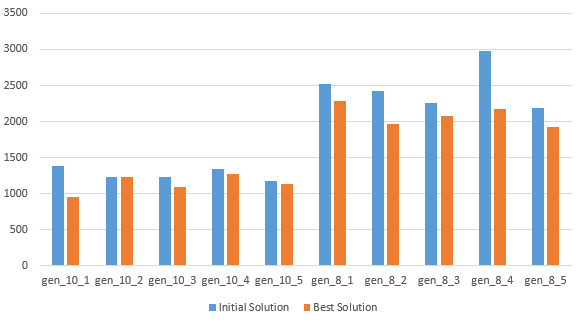
\includegraphics[width=0.8\textwidth]{files/performance_lns.png}
\caption{Performance of our LNS approach}
\label{fig:performance}
\end{figure}



\newpage
\section{Literature}
$[HoMu 12]$ M. I. Hosny and C. L.Mumford, “Constructing initial solutions for the multiple vehicle pickup and delivery problem with time windows”, Journal of King Saud University, Computer and Information Sciences, vol. 24, no. 1, pp. 59–69, 2012.
\\
\\
$[JaHe 11]$ S. Jain , P. Van Hentenryck, “Large neighborhood search for dial-a-ride problems”, In: Principles and practice of constraint programming, Notes in computer science, vol. 6876. Springer, 2011.
\\
\\
$[CoLa 03]$ J.-F. Cordeau, G. Laporte, "A tabu search heuristic for the static multi- vehicle dial-a-ride problem", Transportation Research Part B 37: 579–594, 2003
\\
\\
$[Parragh$  $et$  $al.$ $10]$ S.N. Parragh, K.F. Doerner, R.F. Hartl, "Variable neighborhood search for the dial-a-ride problem", Computers \& Operations Research 37 (6),1129–1138, 2010. 
\\
\\
$[Jørgensen$ $et$ $al.$ $07]$ R.M. Jørgensen , J. Larsen, K.B. Bergvinsdottir, "Solving the dial-a-ride problem using genetic algorithms", J Oper Res Soc 58:1321–1331, 2007.
\end{document}